\documentclass[paper=a4,pagesize=auto,11pt,twoside=true,parskip=half,abstract=on,bibliography=totoc]{report}
\usepackage[T1]{fontenc}
\usepackage{microtype}
\usepackage{graphicx}
\usepackage{appendix}
\usepackage{chngcntr}
\usepackage{hyperref}
%\usepackage{color}
\usepackage[usenames,dvipsnames]{color} 
\usepackage[english,french]{babel}
\usepackage{listings}
\lstset{ 
  language=R,                     % the language of the code
  basicstyle=\small\ttfamily, % the size of the fonts that are used for the code
  numbers=left,                   % where to put the line-numbers
  numberstyle=\small\color{Blue},  % the style that is used for the line-numbers
  stepnumber=1,                   % the step between two line-numbers. If it is 1, each line
                                  % will be numbered
  numbersep=5pt,                  % how far the line-numbers are from the code
  backgroundcolor=\color{white},  % choose the background color. You must add \usepackage{color}
  showspaces=false,               % show spaces adding particular underscores
  showstringspaces=false,         % underline spaces within strings
  showtabs=false,                 % show tabs within strings adding particular underscores
  frame=single,                   % adds a frame around the code
  rulecolor=\color{black},        % if not set, the frame-color may be changed on line-breaks within not-black text (e.g. commens (green here))
  tabsize=2,                      % sets default tabsize to 2 spaces
  captionpos=b,                   % sets the caption-position to bottom
  breaklines=true,                % sets automatic line breaking
  breakatwhitespace=false,        % sets if automatic breaks should only happen at whitespace
  keywordstyle=\color{RoyalBlue},      % keyword style
  commentstyle=\color{YellowGreen},   % comment style
  stringstyle=\color{ForestGreen}      % string literal style
}
\usepackage{amsmath,amsfonts,amssymb}
\usepackage{fontenc}
\usepackage[utf8]{inputenc}%%%%%%%%%%%%%%%%%%%%%%%%%%%%%%%%%%%%%%%%%%%%%%%%%%%
\usepackage[final]{pdfpages} 
\usepackage{float}
\usepackage{amsthm}
\usepackage{pgfplots}
\usepackage{pgfplotstable}
\usepackage{fancyhdr}
\usepackage{dsfont}
\usepackage{comment}
\usepackage[a4paper, hmargin=30mm, vmargin=50mm]{geometry}
%\usepackage{fancyref}
%% Mise en page des théorèmes, lemme etc...


\newtheorem{theorem}{Théorème}[chapter]
\newtheorem{corollary}{Corollaire}[theorem]
\newtheorem{lemma}[theorem]{Lemme}


\theoremstyle{plain}

\newtheorem{thm}{Théorème}[chapter]
%\newtheorem{lemma}{Lemme}[chapter]
%\newtheorem{proof}{Preuve}
%\theoremstyle{prop}
\newtheorem{prop}{Proposition}[chapter]
\newtheorem{cor}{Corollaire}
\theoremstyle{definition}
\newtheorem{definition}{Définition}[chapter]
%\newtheorem{defn}{Définition}[chapter]
%\newtheorem{conj}{Conjecture}[chapter]
\newtheorem{exmp}{Exemple}[chapter]
\theoremstyle{remark}
\newtheorem{remark}{Remarque}
\newtheorem{note}{Note}
\newtheorem{case}{Cas particulier}
%\theoremstyle{Proof}
\newtheorem{Proof}{Preuve}[chapter]
\renewcommand{\floatpagefraction}{0.95}
\renewcommand{\textfraction}{0.05}

\newcommand{\HRule}{\rule{\linewidth}{0.5mm}}

\usepackage{tikz}
\usepackage{pgfplots}
%\usepackage[engilsh]{babel}
\usepackage{csquotes}
\usepackage[section]{placeins}
\usepackage[backend=biber,style=ieee]{biblatex}
\addbibresource{references.bib}

\usepackage{cleveref}
%\hypersetup{
%    hyperfigures = true,
%    colorlinks = true,
%    linkcolor=green
%    }
    
\setcounter{topnumber}{9}
\setcounter{bottomnumber}{9}
\setcounter{totalnumber}{20}
\setcounter{dbltopnumber}{9}


\renewcommand{\H}{\mathcal H}
\providecommand{\R}{\mathbb R}
\providecommand{\N}{\mathbb N}
\providecommand{\prs}[2]{\langle #1, #2\rangle}
\begin{document}
\begin{titlepage}
  \begin{sffamily}
  \begin{center}
    \textsc{\LARGE Université de Montpellier}\\[2cm]
    
\includegraphics[scale=2]{logo-um.png}~\\[1.5cm]
    \textsc{\LARGE Analyse des Données Multidimensionnelles}\\[1.5cm]

    \HRule \\[0.3cm]
    { \huge\bfseries - TP 0 -
    
    Quelques manipulations élémentaires autour de l'inertie 
    
    (des vins de Loire) \\[0.4cm] }
    \HRule \\[2cm]
    \begin{minipage}{0.4\textwidth}
      \begin{center} \large
         \textsc{KANDOUCI Walid}\\
      \end{center}
    \end{minipage}


    \vfill

    % Bottom of the page
    {\large 2019 - 2020}

  \end{center}
  \end{sffamily}
\end{titlepage}

\tableofcontents
\listoffigures
%\chapter*{Résumé}
\chapter*{Introduction et Sommaire}
Dans ce TP, nous allons voir, à l'aide du logiciel R, quelques manipulations élémentaire autour de l'inertie sur notre base de données contenant divers information sur les vins provenant de Loire.
Nous allons tous d'abord centrer-réduire nos variables quantitatives et calculer le barycentre du nuage, puis nous allons calculer les normes euclidiennes  de nos 3 types de vins (Bourgeuil, Chinon, Sammur). Nous allons calculer aussi l'inertie inter-appelation, Le $R^2$ de nos vins.

Enfin, nous allons voir aussi les variables les plus liées à l'appellation ainsi que voir que le $R^2$ de la partition est égal à la moyenne arithmétique des $R^2$ des variables.
\chapter{Quelques manipulations élémentaires
autour de l'inertie (des vins de Loire)}
\section{Notre Base de Données}
Nous allons utilisé la base de données \textbf{"wine.csv"} contenant les données relatives aux vin de la Loire, elle contient deux variables qualitatives:
\begin{itemize}
    \item \textbf{Label:} Bourgueil, Chinon, Saumur
    \item \textbf{Soil:} Env1, Env2, Env3=référence, Env4
\end{itemize}
ainsi que 29 variables quantitatives décrivant diverses intensités sensorielles:  \textbf{Odor Before Shaking, Aroma Before Shaking, Fruity Before Shaking, Flower Before Shaking, Spice Before Shaking, Visual Intensity, Nuance, Surface Feeling, Odor Intensity, Quality of Odour, Fruity, Flower, Spice, Plante, Phenolic, Aroma Intensity, Aroma Persistency, Aroma Quality, Attack Intensityn, Acidity, Astringency, Alcohol, Balance, Smooth, Bitterness, Intensity, Harmony, Overall Quality, Typical}

\section{Centrer-réduire les variables quantitatives}

Nous allons centrer-réduire les variables quantitatives à l'aide de la fonction \textbf{"scale"} comme suit:

\begin{figure}[h]
\centering
\fbox{

\includegraphics[scale=1]{2.PNG}
}
\caption{Code R: Centrer-réduire les variables}
\end{figure}

\subsection{Barycentre du nuage se trouve-il a l'origine?}

Après avoir centré-réduit les variables quantitatives, on calcul le barycentre du nuage:

\begin{figure}[h]
\centering
\fbox{
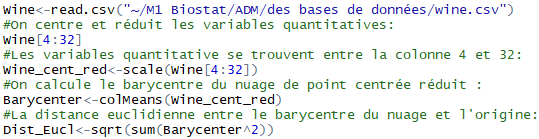
\includegraphics[scale=1]{1.PNG}
}
\caption{Code R: Calcul de du barycentre et de la distance entre le barycentre et l'origine}
\end{figure}

On obtient le résultat suivant:

\begin{figure}[h]
\centering
\fbox{

\includegraphics[scale=1]{4.PNG}
}
\caption{La distance entre le barycentre du nuage et l'origine est presque égal à 0}
\end{figure}

Le barycentre se trouve donc a l’origine.

\subsection{L'inertie totale du nuage est-elle égale au nombre des variables?}

On calcul aussi l’inertie totale du nuage afin de la comparer au nombre des variables:

\begin{figure}[h]
\centering
\fbox{
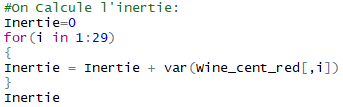
\includegraphics[scale=1]{3.PNG}
}
\caption{Code R: Le Barycentre du nuage se trouve bien à l'origine}
\end{figure}

\newpage

On obtient le résultat suivant:

\begin{figure}[h]
\centering
\fbox{

\includegraphics[scale=1]{5.PNG}
}
\caption{L'inertie total est égal au nombre des variables}
\end{figure}

Donc l'inertie total est égal au nombre des variables.

\section{Calcul des poids et des barycentres des trois appellations (Bourgueil, Chinon, Saumur)}

On calcule les poids des trois appellations \textbf{Chinon, Bourgueil, Saumur}:

\begin{figure}[h]
\centering
\fbox{
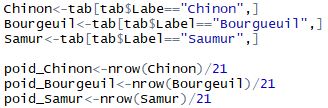
\includegraphics[scale=1]{6.PNG}
}
\caption{Code R -Poids des trois appellations}
\end{figure}

On obtient:

\begin{figure}[h]
\centering
\fbox{

\includegraphics[scale=1]{8.PNG}
}
\caption{Résultats poids des trois appellations}
\end{figure}

Puis, On calcule leurs barycentres:

\begin{figure}[h]
\centering
\fbox{

\includegraphics[scale=1]{7.PNG}
}
\caption{Code R -Barycentres des trois appellations}
\end{figure}

On obtient les résultats suivants:

\begin{figure}[h]
\centering
\fbox{
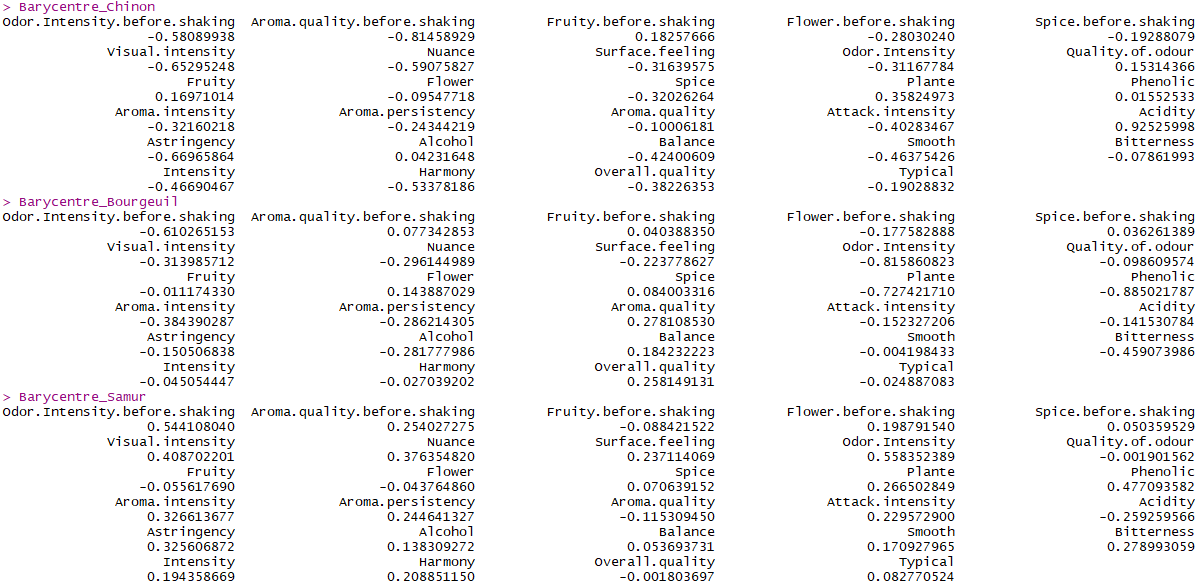
\includegraphics[scale=0.5]{9.PNG}
}
\caption{Résultats Barycentres des trois appellations}
\end{figure}

\newpage

On calcul maintenant les normes euclidiennes carrées de ces trois barycentres et on obtient les résultats suivant:

\begin{figure}[h]
\centering
\fbox{

\includegraphics[scale=0.8]{10.PNG}
}
\caption{Code R et Résultat - Normes euclidiennes carrées des barycentres}
\end{figure}

On en déduit l'inertie inter-appellation:
\begin{figure}[h]
\centering
\fbox{

\includegraphics[scale=0.8]{11.PNG}
}
\caption{Code R et Résultat - Inertie inter-appellation}
\end{figure}

\newpage

Le $R^2$ de la partition des vins en appellations:

\begin{figure}[h]
\centering
\fbox{
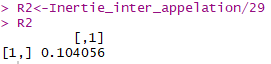
\includegraphics[scale=0.8]{12.PNG}
}
\caption{Code R et Résultat - $R^2$ de la partition des vins en appellations}
\end{figure}

On remarque que $R^2 = 0.104056$ et donc l'appellation n'explique que $11\%$ des disparités sensorielles entre les
vins de Loire.
\section{les variables qui sont les plus liées à l'appellation}
 On cherche & savoir maintenant quelles sont les variables qui sont les plus liées à l'appellation, après avoir calculer le $R^2$ de chaque variable sensorielle, on obtient le résultat suivant:
 
\begin{figure}[h]
\centering
\fbox{
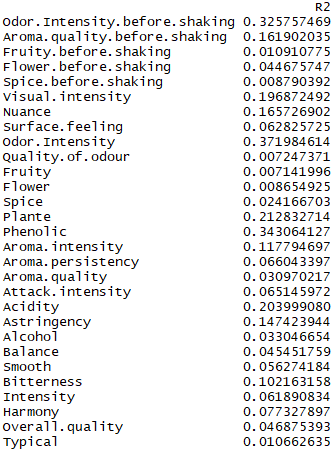
\includegraphics[scale=0.8]{MatriceR2.PNG}
}
\caption{$R^2$ de chaque variable sensorielle}
\end{figure}

On peut conclure alors que les variables les plus liées à l'appellation sont: " Odor.Intensity", "Phenolic", "Odor.Intesity.Before.Shaking", "Plante" et "Acidity".
les moins liées sont: "Fruity", "Quality.Of.odour", "Flower", "Spice.before.shaking" et "Typical".

Pour finir, on calcule la moyenne arithmétique des $R^2$ des variables à l'aide du code suivant, et on obtient:

\begin{figure}[h]
\centering
\fbox{

\includegraphics[scale=0.8]{R222.PNG}
}
\caption{Code R et Résultat - $R^2$ de la partition}
\end{figure}

Ce qui est égale au $R^2$ de la partition.
\chapter*{Conclusion}
Dans ce TP, nous avons eu l'occasion de nous familiariser avec des certaines notions fondamentales de l'analyse des données multidimensionnelles (tel que le calcul des barycentres, le calcul des normes euclidiennes, ainsi que le calcul d'inertie). Ces notions vont nous êtres très utiles pour les TP à venir.
\begin{appendices}
\chapter{Code R TP 0}
\label{Code R} 
\begin{lstlisting} 
# Importation des donnees
Wine<-read.csv("~/M1 Biostat/ADM/des bases de données/wine.csv")
# Centrer reduire les variables quatitatives
Wine_cent_red<-scale(Wine[4:32])
#Barycentre du nuage de point
Barycenter<-colMeans(Wine_cent_red)
# La distance euclidienne entre le barycentre du nuage et l'origine
Dist_Eucl<-sqrt(sum(Barycenter^2))
#Inertie
Inertie=0
for(i in 1:29)
{
Inertie = Inertie + var(Wine_cent_red[,i])
}
# Poids des Appellations
tab<-cbind(Wine[,1:3],Wine_cent_red)
Chinon<-tab[tab$Labe=="Chinon",]
Bourgeuil<-tab[tab$Label=="Bourgueuil",]
Samur<-tab[tab$Label=="Saumur",]
poid_Chinon<-nrow(Chinon)/21
poid_Bourgeuil<-nrow(Bourgeuil)/21
poid_Samur<-nrow(Samur)/21
Poids<-c(poid_Chinon,poid_Bourgeuil,poid_Samur)
Poids
# Barycentre Appellation
Barycentre_Chinon<-colMeans(Chinon[,4:32])
Barycentre_Bourgeuil<-colMeans(Bourgeuil[,4:32])
Barycentre_Samur<-colMeans(Samur[,4:32])
# Normes Euclidiennes
Normes_Eucl<-c(crossprod(Barycentre_Chinon),crossprod(Barycentre_Bourgeuil),crossprod(Barycentre_Samur))
#Inertie Inter
Inertie_inter_appelation<-crossprod(Poids,Normes_Eucl)
#R2
R2<-Inertie_inter_appelation/29
# Nos barycentres
B_Matrix <- matrix(c(Barycentre_Chinon,Barycentre_Bourgeuil,Barycentre_Samur), nrow = 29, ncol = 3)
colnames(B_Matrix) <- c("B.Chinon","B.Bourgueuil","B.Samur")
rownames(B_Matrix) <- c(1:29)
B_Matrix
l = 0
Vec_R2 <- vector(mode ="numeric", length = 29)
for (i in 1:29)
{
N = 0
for (j in 1:3)
{
N = (B_Matrix[i,j])^2*Poids[j] + N
}
l = 1 + l
Vec_R2[l] <- N
}
Matrix_R2 <- matrix(c(Vec_R2), nrow=29, ncol=1, byrow=T)
row.names(Matrix_R2)<-colnames(Wine[,4:32])
colnames(Matrix_R2)<-c("R2")
# R2 = R2
sum(Matrix_R2)/29
\end{lstlisting} 
\end{appendices}

\end{document}